\documentclass[../EDI_Task2_Karwowski_Kowalewski.tex]{subfiles}

\begin{document} {

    \subsection{Przypadek 1 - bazowy} {

        \begin{table}[!htbp]
            \small
            \centering
            \begin{tabular}{|c|c|}
                \hline
                Parametr & Wartość \\ \hline
                outputWordCounts & false \\ \hline
                StopwordsHandler & false \\ \hline
                TFTransform & false \\ \hline
                IDFTransform & false \\ \hline
            \end{tabular}
            \caption{Wartości parametrów dla danej sekcji}
%            \label{}
        \end{table}
        \FloatBarrier

        \subsubsection{Analiza atrybutów} {

            \begin{figure}[!htbp]
                \centering
                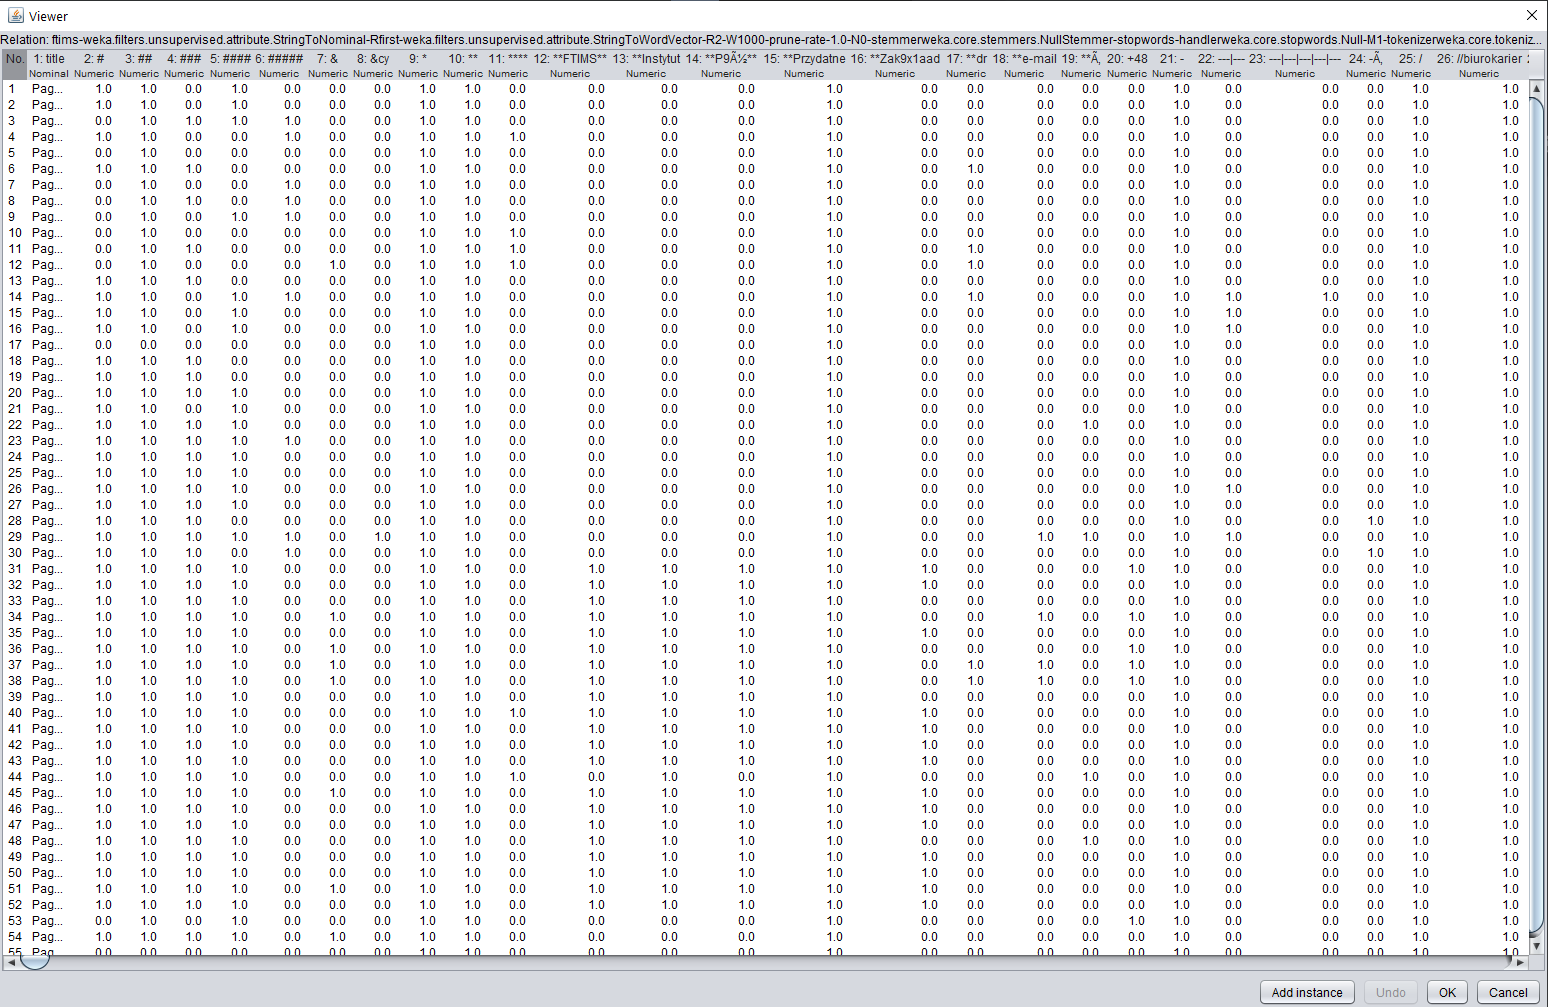
\includegraphics[width=\textwidth]{img/results1/ftims-case1.png}
                \caption{Wyniki analizy atrybutów dla przypadku numer 1}
%                \label{}
            \end{figure}
            \FloatBarrier
        }

        \subsubsection{Analiza klastrowa} {

            \begin{table}[!htbp]
                \small
                \centering
                \begin{tabular}{|c|c|}
                    \hline
                    Klaster & Wartość \\ \hline
                    0   &  19 (35\%) \\
                    1   &   3 (5\%) \\
                    2   &   5 (9\%) \\
                    3   &  17 (31\%) \\
                    4   &   4 (7\%) \\
                    5   &   7 (13\%) \\ \hline
                \end{tabular}
                \caption{Wynik klasteryzacji dla danej sekcji}
%            \label{}
            \end{table}
            \FloatBarrier
        }
    }

    \subsection{Przypadek 2 - outputWordCount} {

        \begin{table}[!htbp]
            \small
            \centering
            \begin{tabular}{|c|c|}
                \hline
                Parametr & Wartość \\ \hline
                outputWordCounts & true \\ \hline
                StopwordsHandler & false \\ \hline
                TFTransform & false \\ \hline
                IDFTransform & false \\ \hline
            \end{tabular}
            \caption{Wartości parametrów dla danej sekcji}
%            \label{}
        \end{table}
        \FloatBarrier

        \subsubsection{Analiza atrybutów} {

            \begin{figure}[!htbp]
                \centering
                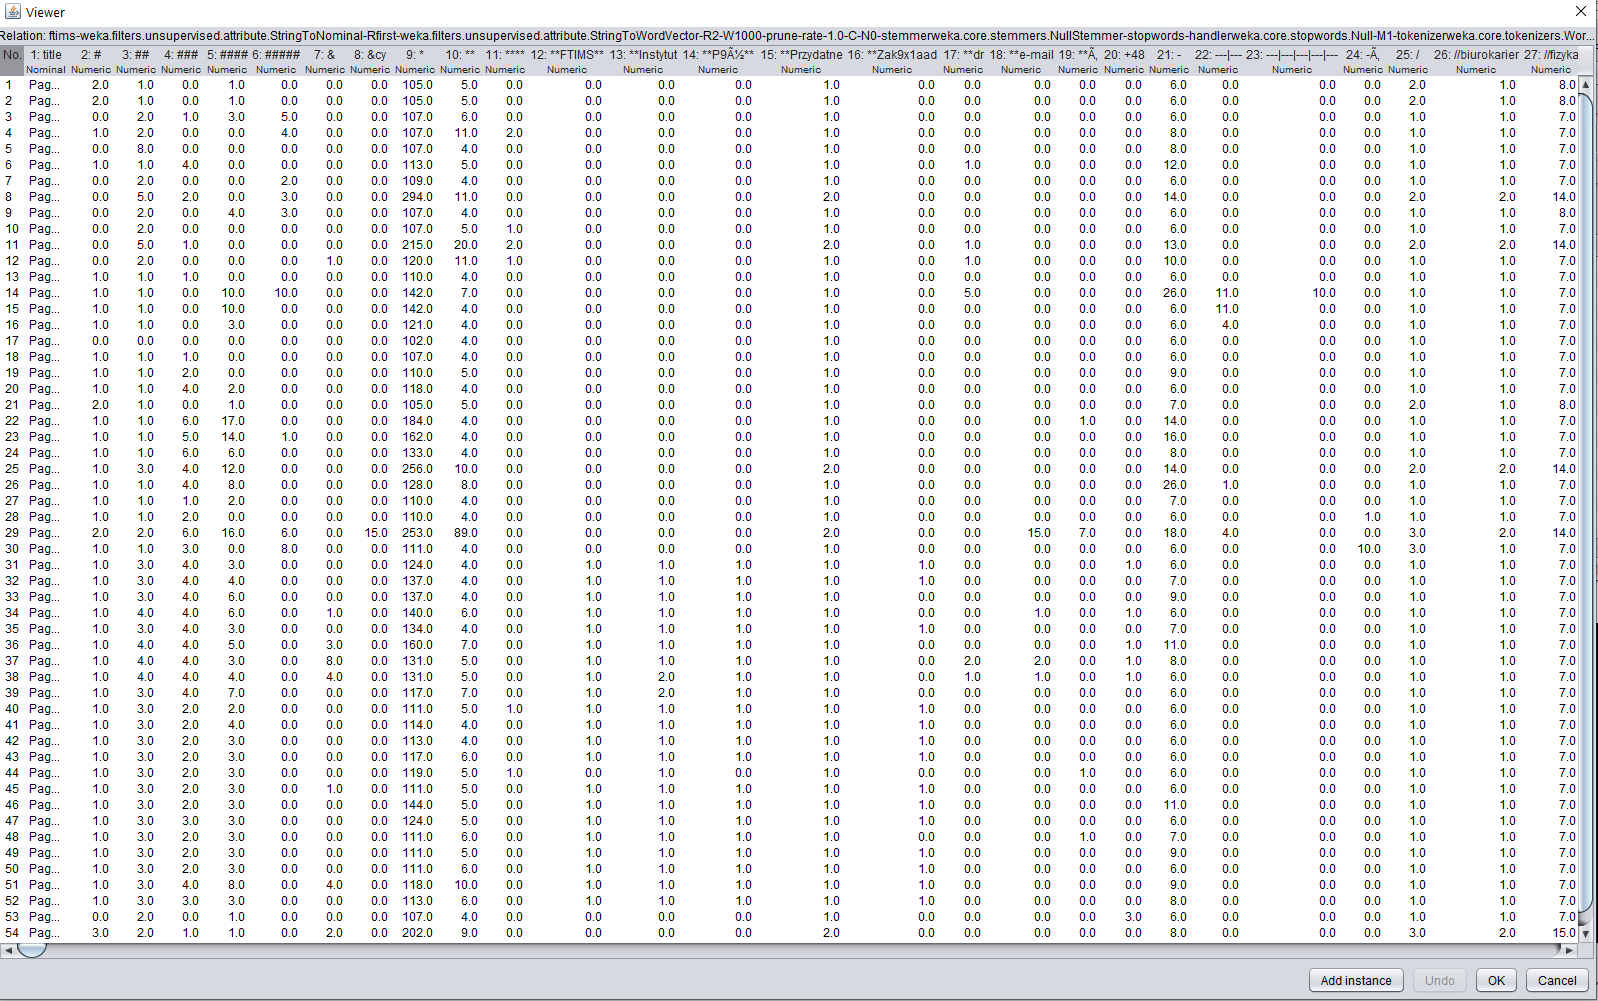
\includegraphics[width=\textwidth]{img/results1/ftims-case2.png}
                \caption{Wyniki analizy atrybutów dla przypadku numer 2}
%                \label{}
            \end{figure}
            \FloatBarrier
        }

        \subsubsection{Analiza klastrowa} {

            \begin{table}[!htbp]
                \small
                \centering
                \begin{tabular}{|c|c|}
                    \hline
                    Klaster & Wartość \\ \hline
                    0   &  55 (100\%) \\ \hline
                \end{tabular}
                \caption{Wynik klasteryzacji dla danej sekcji}
%            \label{}
            \end{table}
            \FloatBarrier
        }
    }

    \subsection{Przypadek 3 - StopwordsHandler} {

        \begin{table}[!htbp]
            \small
            \centering
            \begin{tabular}{|c|c|}
                \hline
                Parametr & Wartość \\ \hline
                outputWordCounts & false \\ \hline
                StopwordsHandler & true \\ \hline
                TFTransform & false \\ \hline
                IDFTransform & false \\ \hline
            \end{tabular}
            \caption{Wartości parametrów dla danej sekcji}
%            \label{}
        \end{table}
        \FloatBarrier

        \subsubsection{Analiza atrybutów} {

            \begin{figure}[!htbp]
                \centering
                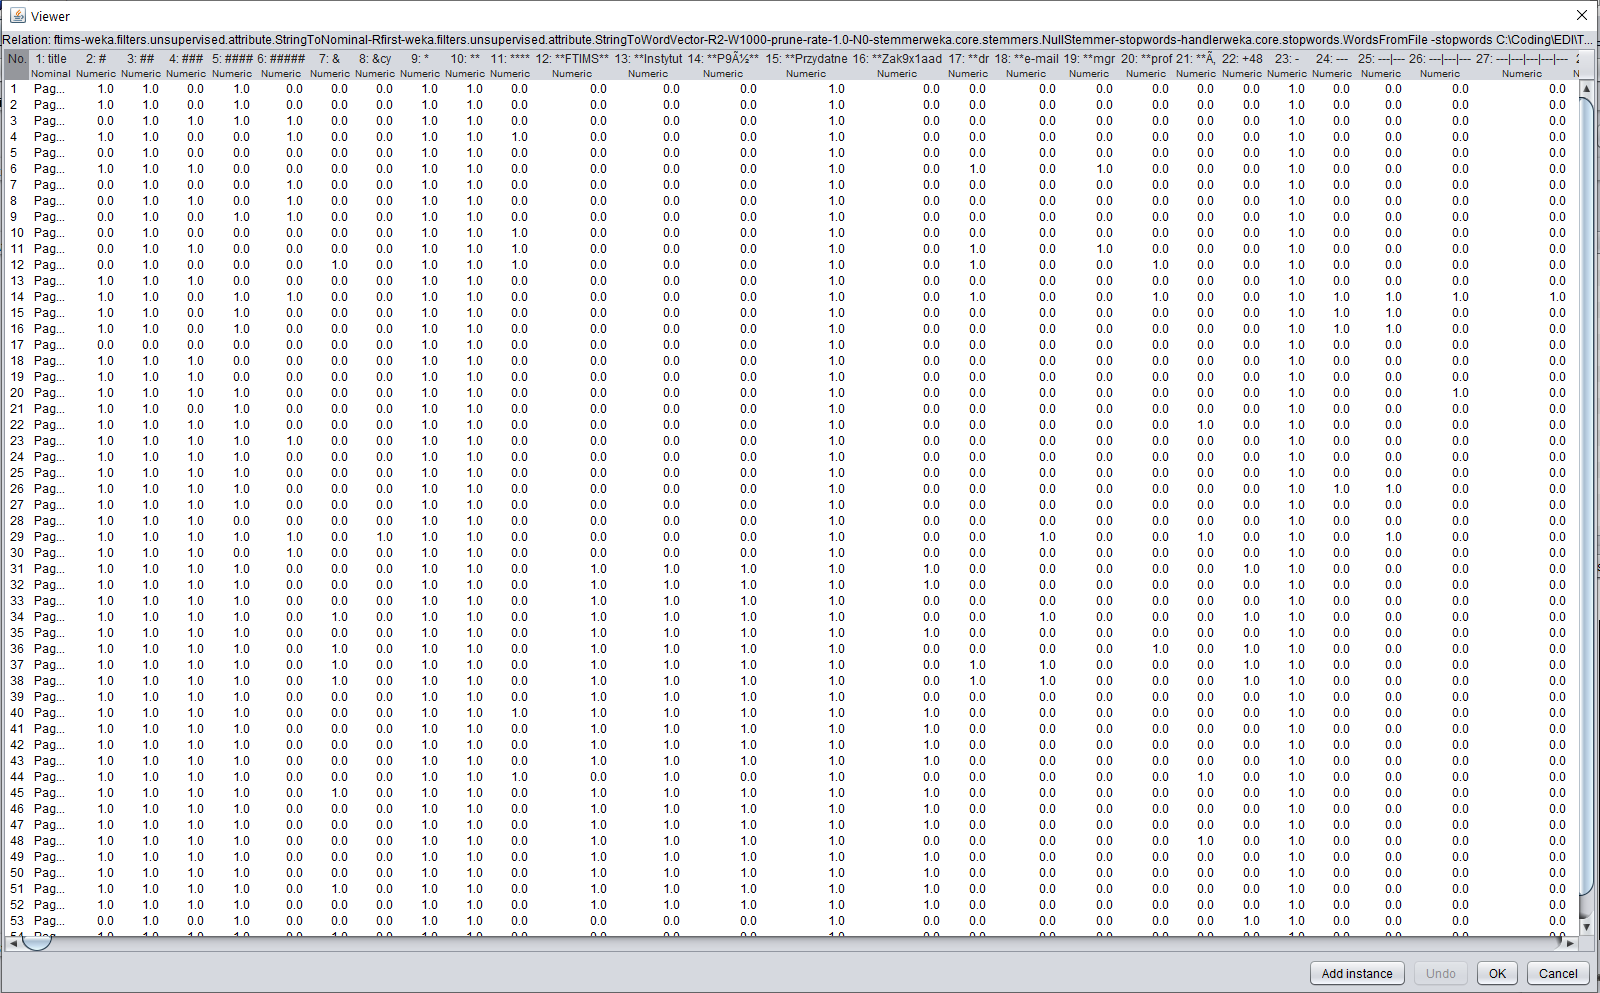
\includegraphics[width=\textwidth]{img/results1/ftims-case3.png}
                \caption{Wyniki analizy atrybutów dla przypadku numer 3}
%                \label{}
            \end{figure}
            \FloatBarrier
        }

        \subsubsection{Analiza klastrowa} {

            \begin{table}[!htbp]
                \small
                \centering
                \begin{tabular}{|c|c|}
                    \hline
                    Klaster & Wartość \\ \hline
                    0   &  37 (67\%) \\
                    1   &   2 (4\%) \\
                    2   &  16 (29\%) \\ \hline
                \end{tabular}
                \caption{Wynik klasteryzacji dla danej sekcji}
%            \label{}
            \end{table}
            \FloatBarrier
        }
    }

    \subsection{Przypadek 4 - TFTransform} {

        \begin{table}[!htbp]
            \small
            \centering
            \begin{tabular}{|c|c|}
                \hline
                Parametr & Wartość \\ \hline
                outputWordCounts & false \\ \hline
                StopwordsHandler & false \\ \hline
                TFTransform & true \\ \hline
                IDFTransform & false \\ \hline
            \end{tabular}
            \caption{Wartości parametrów dla danej sekcji}
%            \label{}
        \end{table}
        \FloatBarrier

        \subsubsection{Analiza atrybutów} {

            \begin{figure}[!htbp]
                \centering
                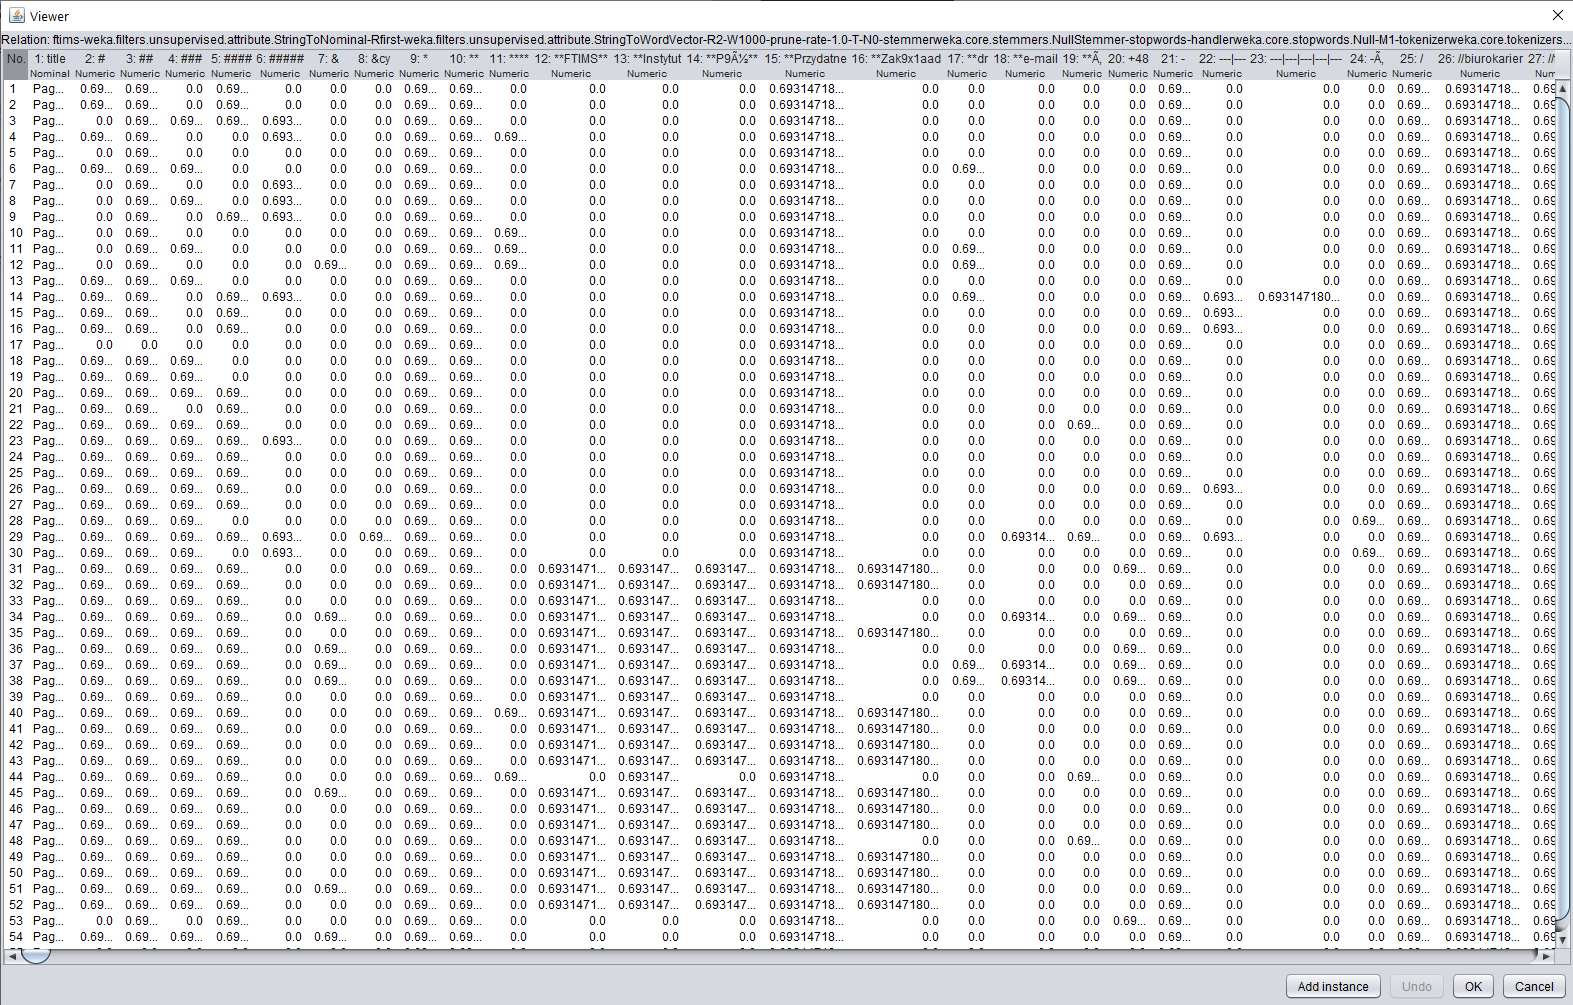
\includegraphics[width=\textwidth]{img/results1/ftims-case4.png}
                \caption{Wyniki analizy atrybutów dla przypadku numer 4}
%                \label{}
            \end{figure}
            \FloatBarrier
        }

        \subsubsection{Analiza klastrowa} {

            \begin{table}[!htbp]
                \small
                \centering
                \begin{tabular}{|c|c|}
                    \hline
                    Klaster & Wartość \\ \hline
                    0   &  19 (35\%) \\
                    1   &   3 (5\%) \\
                    2   &   5 (9\%) \\
                    3   &  17 (31\%) \\
                    4   &   4 (7\%) \\
                    5   &   7 (13\%) \\ \hline
                \end{tabular}
                \caption{Wynik klasteryzacji dla danej sekcji}
%            \label{}
            \end{table}
            \FloatBarrier
        }
    }

    \subsection{Przypadek 5 - IDFTransform} {

        \begin{table}[!htbp]
            \small
            \centering
            \begin{tabular}{|c|c|}
                \hline
                Parametr & Wartość \\ \hline
                outputWordCounts & false \\ \hline
                StopwordsHandler & false \\ \hline
                TFTransform & false \\ \hline
                IDFTransform & true \\ \hline
            \end{tabular}
            \caption{Wartości parametrów dla danej sekcji}
%            \label{}
        \end{table}
        \FloatBarrier

        \subsubsection{Analiza atrybutów} {

            \begin{figure}[!htbp]
                \centering
                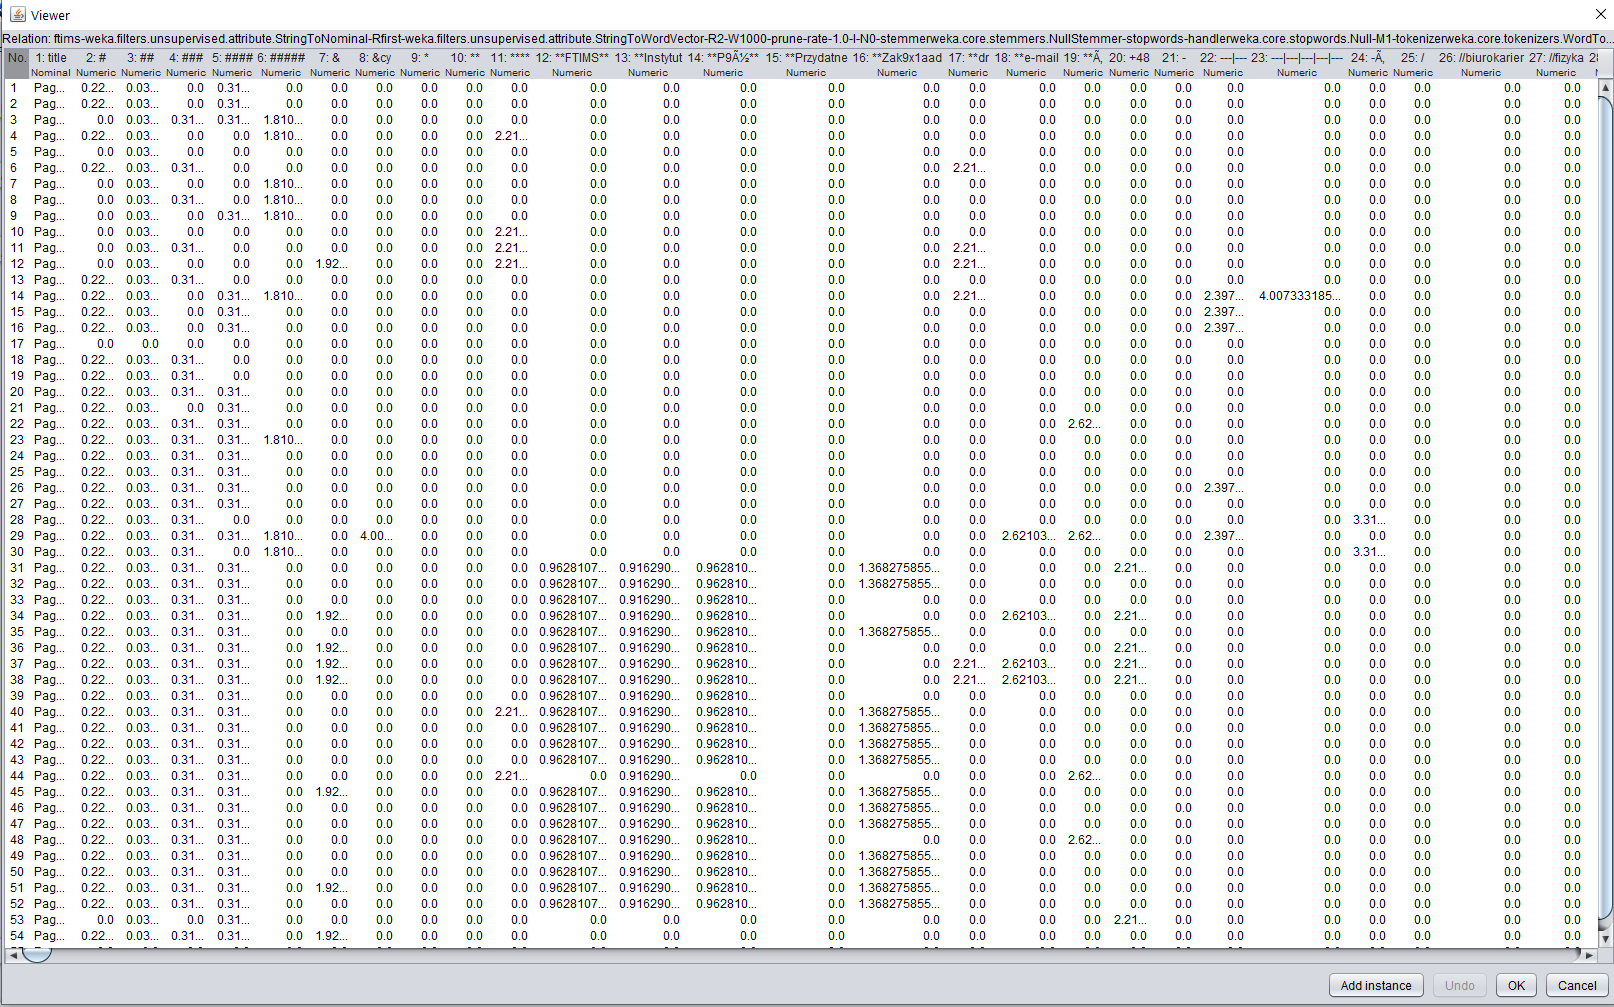
\includegraphics[width=\textwidth]{img/results1/ftims-case5.png}
                \caption{Wyniki analizy atrybutów dla przypadku numer 5}
%                \label{}
            \end{figure}
            \FloatBarrier
        }

        \subsubsection{Analiza klastrowa} {

            \begin{table}[!htbp]
                \small
                \centering
                \begin{tabular}{|c|c|}
                    \hline
                    Klaster & Wartość \\ \hline
                    0   &  19 (35\%) \\
                    1   &   3 (5\%) \\
                    2   &   5 (9\%) \\
                    3   &  17 (31\%) \\
                    4   &   4 (7\%) \\
                    5   &   7 (13\%) \\ \hline
                \end{tabular}
                \caption{Wynik klasteryzacji dla danej sekcji}
%            \label{}
            \end{table}
            \FloatBarrier
        }
    }

    \subsection{Przypadek 6 - TFTransform i IDFTransform} {

        \begin{table}[!htbp]
            \small
            \centering
            \begin{tabular}{|c|c|}
                \hline
                Parametr & Wartość \\ \hline
                outputWordCounts & false \\ \hline
                StopwordsHandler & false \\ \hline
                TFTransform & true \\ \hline
                IDFTransform & true \\ \hline
            \end{tabular}
            \caption{Wartości parametrów dla danej sekcji}
%            \label{}
        \end{table}
        \FloatBarrier

        \subsubsection{Analiza atrybutów} {

            \begin{figure}[!htbp]
                \centering
                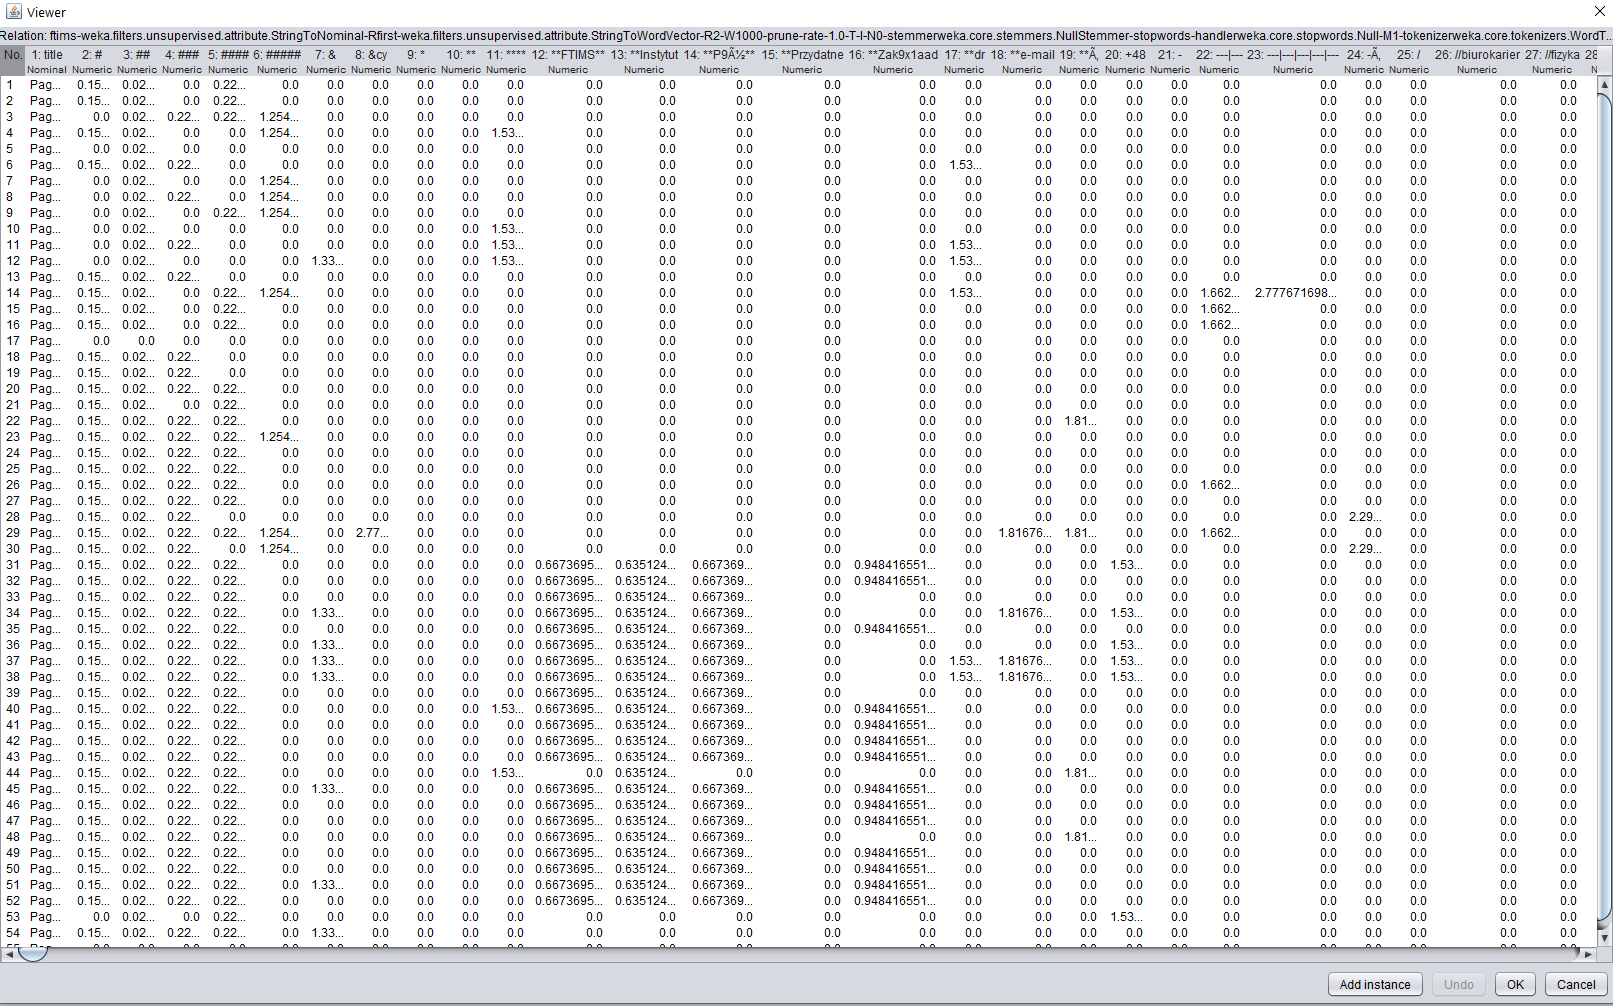
\includegraphics[width=\textwidth]{img/results1/ftims-case6.png}
                \caption{Wyniki analizy atrybutów dla przypadku numer 6}
%                \label{}
            \end{figure}
            \FloatBarrier
        }

        \subsubsection{Analiza klastrowa} {

            \begin{table}[!htbp]
                \small
                \centering
                \begin{tabular}{|c|c|}
                    \hline
                    Klaster & Wartość \\ \hline
                    0   &  19 (35\%) \\
                    1   &   3 (5\%) \\
                    2   &   5 (9\%) \\
                    3   &  17 (31\%) \\
                    4   &   4 (7\%) \\
                    5   &   7 (13\%) \\ \hline
                \end{tabular}
                \caption{Wynik klasteryzacji dla danej sekcji}
%            \label{}
            \end{table}
            \FloatBarrier
        }
    }

    \subsection{Przypadek 7 - TFTransform, IDFTransform i outputWordCounts} {

        \begin{table}[!htbp]
            \small
            \centering
            \begin{tabular}{|c|c|}
                \hline
                Parametr & Wartość \\ \hline
                outputWordCounts & true \\ \hline
                StopwordsHandler & false \\ \hline
                TFTransform & true \\ \hline
                IDFTransform & true \\ \hline
            \end{tabular}
            \caption{Wartości parametrów dla danej sekcji}
%            \label{}
        \end{table}
        \FloatBarrier

        \subsubsection{Analiza atrybutów} {

            \begin{figure}[!htbp]
                \centering
                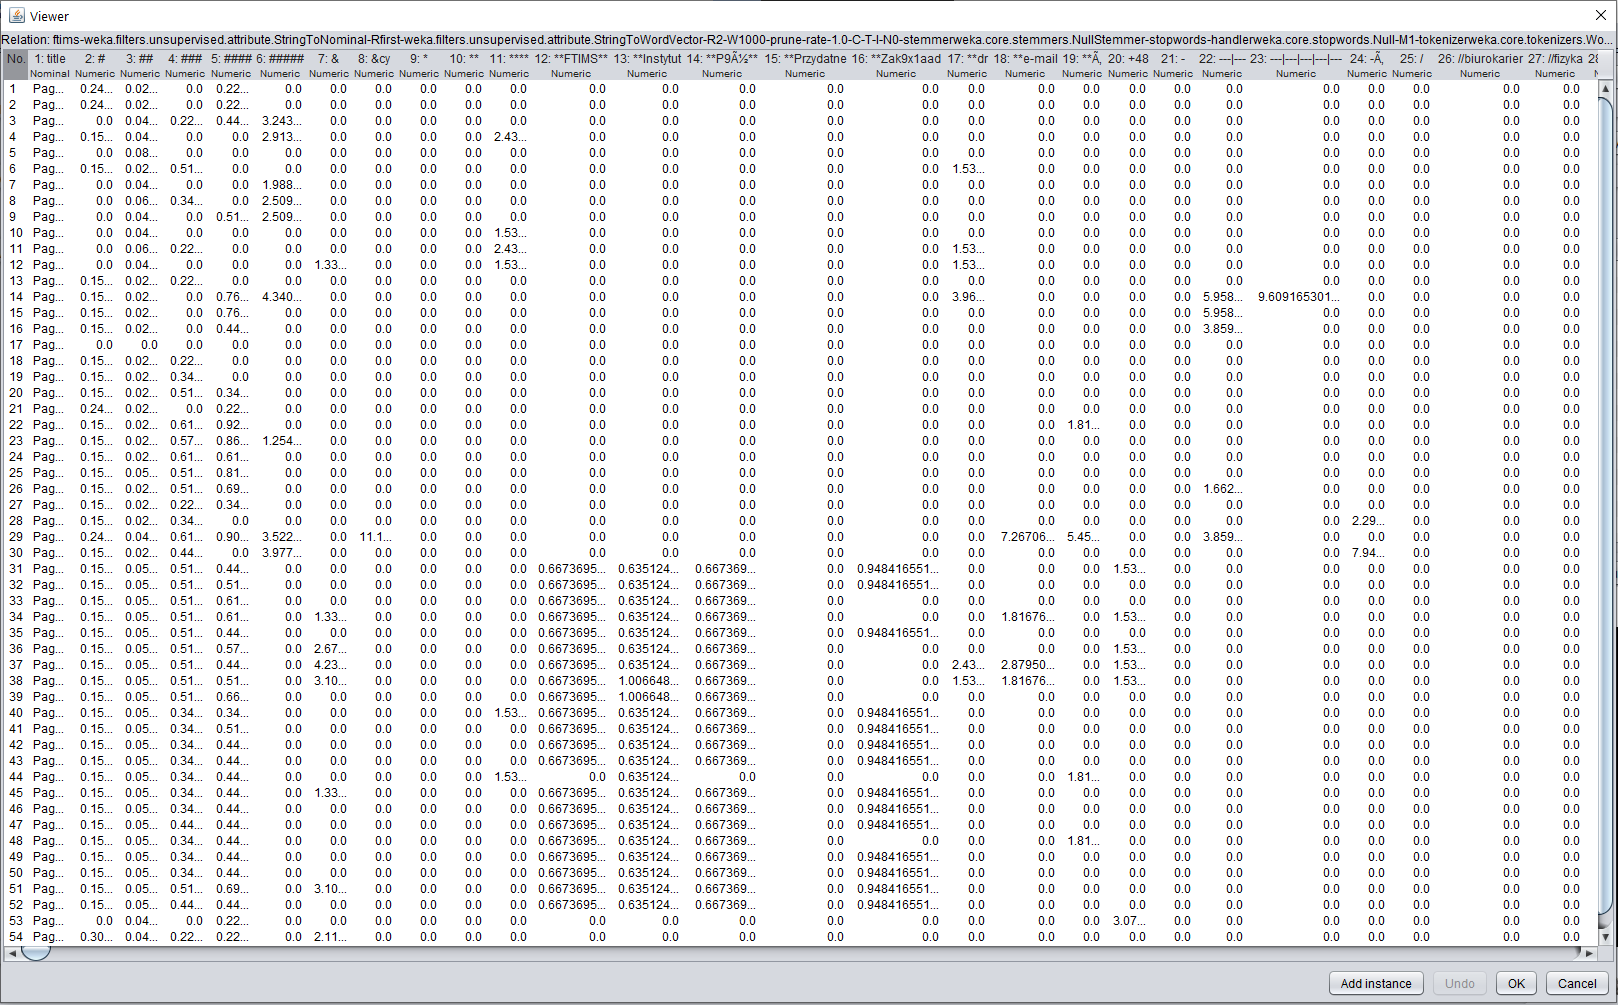
\includegraphics[width=\textwidth]{img/results1/ftims-case7.png}
                \caption{Wyniki analizy atrybutów dla przypadku numer 7}
%                \label{}
            \end{figure}
            \FloatBarrier
        }

        \subsubsection{Analiza klastrowa} {

            \begin{table}[!htbp]
                \small
                \centering
                \begin{tabular}{|c|c|}
                    \hline
                    Klaster & Wartość \\ \hline
                    0   &  16 (29\%) \\
                    1   &   3 (5\%) \\
                    2   &   4 (7\%) \\
                    3   &  18 (33\%) \\
                    4   &   4 (7\%) \\
                    5   &  10 (18\%) \\ \hline
                \end{tabular}
                \caption{Wynik klasteryzacji dla danej sekcji}
%            \label{}
            \end{table}
            \FloatBarrier
        }
    }

    \subsection{Przypadek 8 - Reprezentacja binarna} {

        \begin{table}[!htbp]
            \small
            \centering
            \begin{tabular}{|c|c|}
                \hline
                Parametr & Wartość \\ \hline
                outputWordCounts & false \\ \hline
                StopwordsHandler & false \\ \hline
                TFTransform & false \\ \hline
                IDFTransform & false \\ \hline
            \end{tabular}
            \caption{Wartości parametrów dla danej sekcji}
%            \label{}
        \end{table}
        \FloatBarrier

        \subsubsection{Analiza atrybutów} {

            \begin{figure}[!htbp]
                \centering
                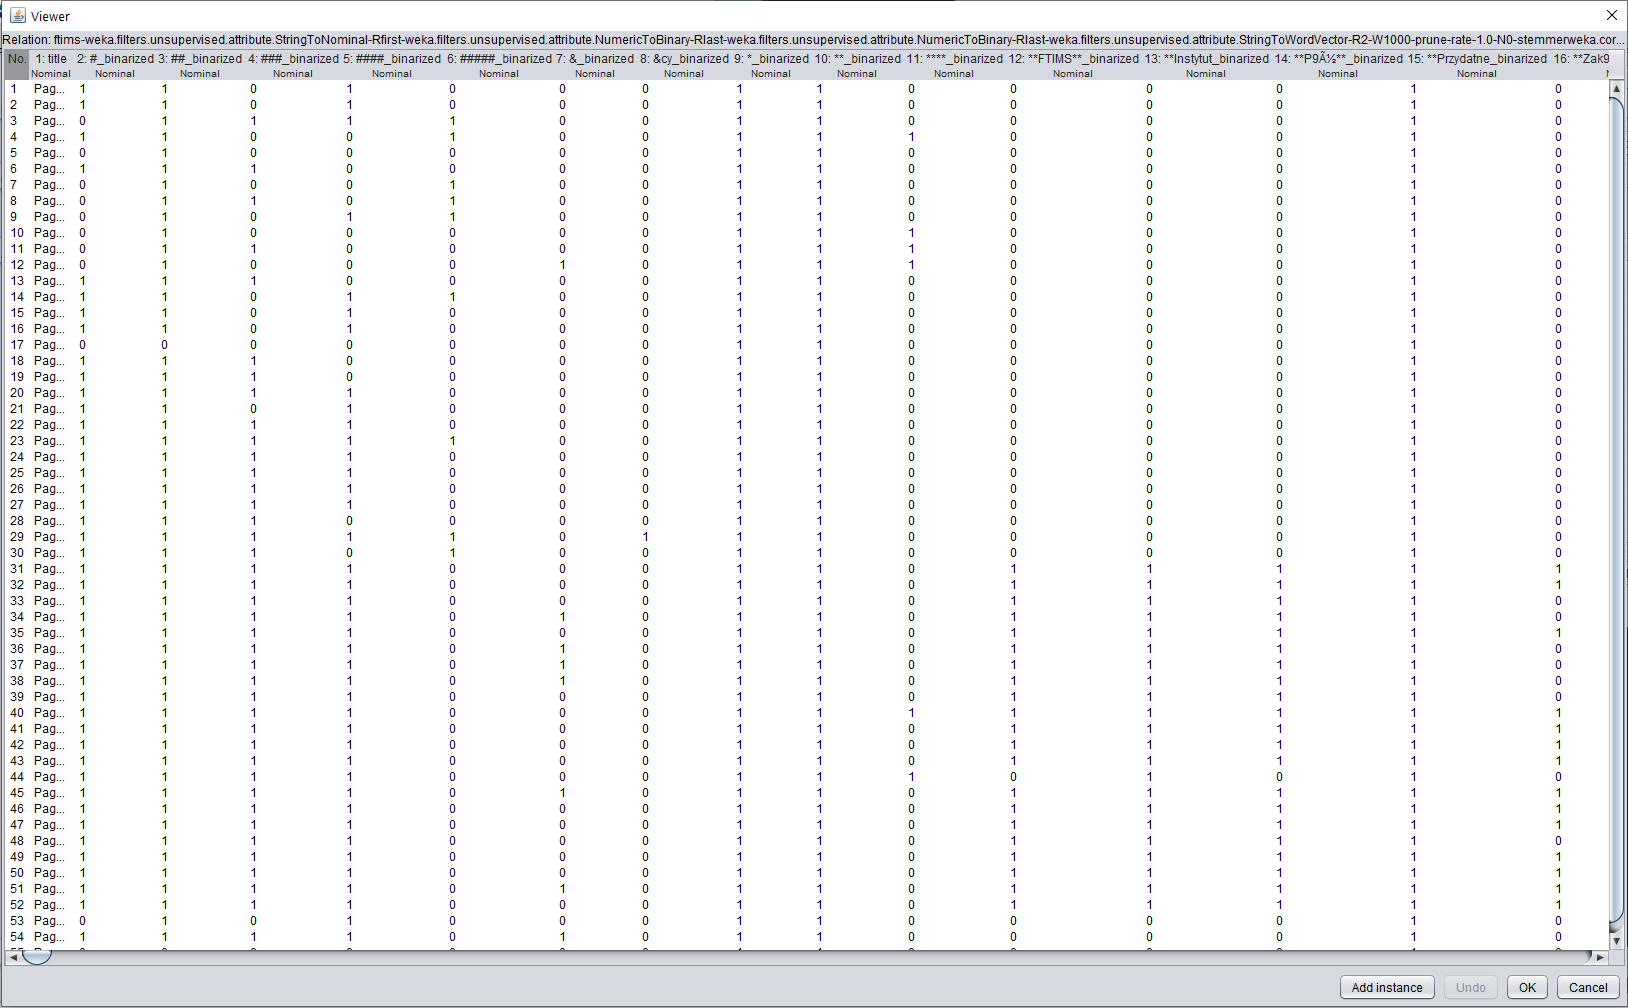
\includegraphics[width=\textwidth]{img/results1/ftims-case8.png}
                \caption{Wyniki analizy atrybutów dla przypadku numer 8}
%                \label{}
            \end{figure}
            \FloatBarrier
        }

        \subsubsection{Analiza klastrowa} {

            \begin{table}[!htbp]
                \small
                \centering
                \begin{tabular}{|c|c|}
                    \hline
                    Klaster & Wartość \\ \hline
                    0   &  13 (24\%) \\
                    1   &  16 (29\%) \\
                    2   &   3 (5\%) \\
                    3   &   9 (16\%) \\
                    4   &   9 (16\%) \\
                    5   &   5 (9\%) \\ \hline
                \end{tabular}
                \caption{Wynik klasteryzacji dla danej sekcji}
%            \label{}
            \end{table}
            \FloatBarrier
        }
    }
}
\end{document}
